\documentclass[dvipsnames]{article}

\usepackage{tikz}
\usepackage{pgfplots,pgfplotstable}
\pgfplotsset{compat=newest}
\usepgfplotslibrary{external}
\tikzexternalize
\usetikzlibrary{shapes,patterns.meta}

\tikzsetexternalprefix{frames/}
\pgfkeys{/pgf/number format/.cd,int detect,1000 sep={\,},min exponent for 1000 sep=4}

\begin{document}
\newcounter{nodelabel}
\foreach \s [count=\iter] in {0,0.05,...,1.95}{
	
\pgfmathsetbasenumberlength{3}
\pgfmathsetcounter{nodelabel}{\iter}
\pgfmathbasetodec\nodelabel{\the\value{nodelabel}}{10}%
\tikzsetnextfilename{frame\nodelabel}

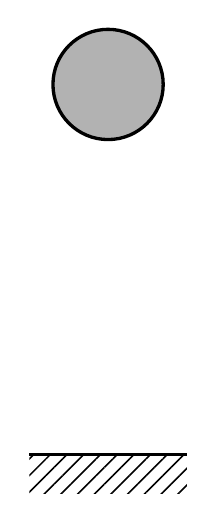
\begin{tikzpicture}
	% ball
	\draw[draw=black,very thick,fill=black!30] (1,{4-4*(1-abs(\s-1))^2}) ellipse (0.7 and 0.7);
	% ground
	\path[draw=none,postaction={pattern={Lines[angle=45,line width=0.2mm,distance=1.5mm]},pattern color = black}] (0,-0.7) -- (2,-0.7) --++ (0,-0.5) --++ (-2,0) -- cycle;
	\path[draw=black,fill=none,very thick] (0,-0.7) -- (2,-0.7);
	% background
	\path[draw=none,fill=none] (0,-0.7) -- (2,-0.7) --++ (0,5.4) --++ (-2,0) -- cycle;
\end{tikzpicture}
}
\end{document}